\documentclass[11pt]{article}
\usepackage[T1]{fontenc}
\usepackage[utf8]{inputenc}
\usepackage{lmodern}
\usepackage[margin=1in]{geometry}
\usepackage{amsmath,amssymb,amsthm,mathtools}
\usepackage{enumitem,microtype}
\usepackage{xcolor,tikz}
\usetikzlibrary{arrows.meta,positioning}
\usepackage[colorlinks=true,linkcolor=blue!45!black,citecolor=blue!45!black,urlcolor=blue!45!black]{hyperref}
\usepackage{bookmark}
\hypersetup{pdftitle={Sharp Pathwidth Bounds for the Permanent, Hamiltonian Cycles, and the Tutte Polynomial}}
\definecolor{ink}{HTML}{233748}
\definecolor{sea}{HTML}{26736E}
\definecolor{ochre}{HTML}{A46325}
\newtheorem{theorem}{Theorem}[section]
\newtheorem{lemma}[theorem]{Lemma}
\newtheorem{proposition}[theorem]{Proposition}
\theoremstyle{definition}
\newtheorem{example}[theorem]{Example}
\newcommand{\F}{\mathbb F}
\newcommand{\pw}{\operatorname{pw}}
\newcommand{\per}{\operatorname{per}}
\newcommand{\hc}{\operatorname{hc}}
\newcommand{\rank}{\operatorname{rank}}
\newcommand{\id}{\mathrm{id}}
\newcommand{\one}{\mathbf{1}}
\newcommand{\OO}{O^*}
\newcommand{\bits}{\{0,1\}}
\newcommand{\olF}{\overline{\F}}
\newcommand{\angles}[1]{\left\langle #1\right\rangle}
\newcommand{\circuit}{\mathsf{size}}
\DeclareMathOperator{\End}{End}
\DeclareMathOperator{\tr}{tr}
\setlist{topsep=4pt,itemsep=2pt}
\title{Sharp Pathwidth Bounds for the Permanent,\\ Hamiltonian Cycles, and the Tutte Polynomial}
\author{}
\date{}

\begin{document}
\maketitle
\vspace{-2.8em}
\begin{abstract}
We prove unconditional arithmetic circuit lower bounds in terms of the pathwidth \(p\) of the support graph. Over every field of characteristic different from two, for every \(0<\varepsilon<1\) and \(C\ge0\), there are bipartite graphs of maximum degree three whose permanent requires more than \(n^C(2-\varepsilon)^p\) gates, where \(n=1+|V|+|E|\). The matching upper bound is \(n^{O(1)}2^p\). For the directed Hamiltonian cycle polynomial the optimal base is six outside characteristic two and \(2+2\sqrt2\) in characteristic two. For the multivariate Tutte cluster polynomial with an indeterminate cluster parameter, every fixed saving in the leading exponent \(p\log_2 p\) is impossible over every field. We also determine the optimal base when the parameter is a fixed number of colors.
\end{abstract}

\section{Introduction}

A perfect matching meets every vertex exactly once. To compute its generating polynomial along a path decomposition, it suffices to remember which vertices in the current bag have already been matched. Could an arithmetic circuit save a fixed fraction of these bits by reusing intermediate results or using cancellation? The first theorem gives an unconditional lower bound even for circuits designed separately for each graph.

Write \(s_{\F}(f)\) for the minimum number of binary \(+,-,\times\) gates needed to compute the formal polynomial \(f\) over the field \(\F\). Variables and arbitrary field constants are free inputs. The circuit may have arbitrary depth and reuse any gate output. A path decomposition of a graph is a sequence of vertex sets, called bags, in which each vertex occurs on a nonempty interval and the ends of every edge occur together in some bag. The pathwidth \(\pw(G)\) is the minimum, over such decompositions, of the largest bag size minus one.

For a bipartite graph \(G=(V,E)\), give each edge its own indeterminate \(x_e\). Its permanent is \(\per(G)=\sum_M\prod_{e\in M}x_e\), summed over all perfect matchings \(M\). Put \(p=\pw(G)\) and \(n=1+|V|+|E|\).

\begin{theorem}[Permanent]\label{thm:permanent}
Over every field \(\F\) of characteristic different from two, for every \(0<\varepsilon<1\) and \(C\ge0\), there are bipartite graphs of maximum degree three and arbitrarily large \(p\) for which
\[
                     s_{\F}(\per(G))>n^C(2-\varepsilon)^p .
\]
For every bipartite graph, \(n^{O(1)}2^p\) gates suffice. In characteristic two, \(n^{O(1)}\) gates suffice for every bipartite graph.
\end{theorem}

For a directed graph \(G=(V,A)\), let \(\hc(G)=\sum_H\prod_{a\in H}x_a\), with one indeterminate per arc and one term per spanning directed cycle, counted up to cyclic rotation. Let \(p\) be the pathwidth of the underlying undirected graph and put \(n=1+|V|+|A|\).

\begin{theorem}[Directed Hamiltonian cycle]\label{thm:tours}
Fix a field \(\F\). Set \(b=6\) if its characteristic differs from two and \(b=2+2\sqrt 2\) if its characteristic is two. For every \(0<\varepsilon<b-1\) and \(C\ge0\), there are directed graphs of arbitrarily large \(p\), with all indegrees and outdegrees at most three, for which
\[
                       s_{\F}(\hc(G))>n^C(b-\varepsilon)^p .
\]
For every directed graph, \(\hc(G)\) has a circuit over \(\F\) of size \(n^{O(1)}b^p\).
\end{theorem}

In both theorems the hard graphs can be chosen with \(\log n=o(p)\). A fixed saving in the exponential base therefore outweighs any fixed polynomial factor in graph size. The path decomposition can be supplied with the graph.

The multivariate Tutte polynomial records the connected components of every spanning subgraph~\cite{sokal}. Its width dependence changes when the cluster parameter is specialized to an integer.

Let \(G=(V,E)\) be a loopless undirected graph, \(p=\pw(G)\), and \(n=1+|V|+|E|\). With \(Q\) and the edge weights \(w_e\) independent indeterminates, set
\begin{equation}\label{eq:cluster}
 Z_G(Q,\mathbf w)=\sum_{A\subseteq E}Q^{\kappa(V,A)}\prod_{e\in A}w_e ,
\end{equation}
where \(\kappa(V,A)\) counts the connected components of \((V,A)\), including isolated vertices.

\begin{theorem}[Tutte cluster polynomial]\label{thm:cluster}
Over every field \(\F\), for every \(0<\varepsilon<1\) and \(C\ge0\), there are graphs of arbitrarily large \(p\) for which
\[
             s_{\F}\bigl(Z_G(Q,\mathbf w)\bigr)>n^C\,2^{(1-\varepsilon)p\log_2 p}.
\]
For every graph a circuit of size \(n^{O(1)}\operatorname{Bell}(p+1)\) suffices, where \(\operatorname{Bell}(k)\) counts the partitions of a \(k\)-element set.
\end{theorem}

Fix an integer \(q\ge1\) and a field \(\F\). For a loopless undirected graph \(G=(V,E)\), the specialization \(Z_G(q,-\mathbf y)\) is the unique polynomial multilinear in the edge indicators \(y_e\) whose value at \(\mathbf1_A\) is the number of proper \(q\)-colorings of \((V,A)\), evaluated in \(\F\). Put \(p=\pw(G)\) and \(n=1+|V|+|E|\).

\begin{theorem}[Fixed number of colors]\label{thm:color}
Let \(r=q\) in characteristic zero and let \(r\) be the least nonnegative residue of \(q\) modulo the characteristic otherwise. If \(r\ge2\), then for every \(0<\varepsilon<r-1\) and \(C\ge0\) there are graphs of arbitrarily large \(p\) for which
\[
                      s_{\F}\bigl(Z_G(q,-\mathbf y)\bigr)>n^C(r-\varepsilon)^p .
\]
Every graph admits a circuit of size \(n^{O(1)}r^p\) in this case. For \(r=0\) the polynomial vanishes on every graph with at least one vertex. For \(r=1\) it equals \(\prod_{e\in E}(1-y_e)\). The empty graph gives one in all cases.
\end{theorem}

All four circuit lower bounds are unconditional. They follow from the Euclidean price theorem of OpenAI~\cite{euclid}. They also hold for border circuits in the sense of Section~\ref{sec:tables}, and with treewidth in the lower-bound exponents since treewidth is at most pathwidth. In the proofs, \(\OO\) suppresses a fixed polynomial in \(n\).

\paragraph{Where the bases come from.}
Suppose a table on each vertex of a graph reads the labels on its incident edges. We construct an ordered graph for which summing the product of the tables needs nearly \(2^A\) gates, where \(A\) is the largest number of bits crossing a cut in the order. The price theorem of OpenAI~\cite{euclid} supplies the circuit lower bound. A power of a path supplies demands for which \emph{every} balanced cut is as expensive as the most expensive prefix. Routing these demands on a strip makes individual tables small. We give the construction in Section~\ref{sec:tables}.

It remains to put as many labels as possible on a boundary of \(m\) vertices. Half-size subsets suffice for perfect matchings, giving \(2^{m-o(m)}\) labels. For directed tours a boundary specifies degrees and a pairing of path ends. The rank of the pairing test gives \(6^{m-o(m)}\) labels in odd or zero characteristic. For named colors a boundary simply stores a word in \([q]^m\). Section~\ref{sec:color} shows how to read an arbitrary table of such words. With an indeterminate cluster parameter, a clique names enough colors to store almost \(\log_2 p\) bits at a single boundary vertex.

OpenAI use balanced circuit cuts and sparse graph projections for the permanent and the directed Hamiltonian cycle polynomial~\cite{circuits}. Our width estimates use their circuit argument and several of their local gadgets. Molter's encoding of choices into bits~\cite{molter} and the use of routings to measure graph cuts by Curticapean, Döring, Neuen, and Wang~\cite{linkup} suggest the two parts of the construction. Their decision-time hypotheses play no role here. For tours, the use of the rank of a matching compatibility matrix goes back to work of Cygan, Kratsch, and Nederlof~\cite{ckn} and Curticapean, Lindzey, and Nederlof~\cite{cln}. We will need the bipartite permutation version of this matrix.

\section{A family of hard tables}\label{sec:tables}

For a graph \(H\), give edge \(e\) a label of \(c_e\) bits. At vertex \(v\), introduce a separate indeterminate \(X_{v,\alpha}\) for every possible joint label \(\alpha\) on its incident edges \(\delta(v)\). Define
\begin{equation}\label{eq:source}
 F_H=\sum_{\sigma\in\prod_e\bits^{c_e}}\ \prod_{v\in V(H)}X_{v,\sigma|_{\delta(v)}}.
\end{equation}
Given an order on \(V(H)\), let \(A\) be the largest total \(c_e\) crossing a prefix, and \(T=\max_v\sum_{e\ni v}c_e\). Reading the tables in order computes \(F_H\) with \(2^A\) times a polynomial in the input-table length many operations. We shall use the following converse on a particular family.

\begin{proposition}\label{prop:hard}
For every \(\eta>0\) there are ordered graphs \(H\) and numbers \(D\to\infty\) with
\[
 A\le(1+\eta)D,\qquad T=o(D),\qquad
 \log_2(\circuit(F_H)+1)\ge (1-o(1))D.
\]
The size here can be degree-component border size over any field. The graphs have polynomially many vertices and edges in \(D\). The maximum unweighted degree and the maximum number of edges crossing a prefix are both \(o(D)\).
\end{proposition}

For a homogeneous polynomial of degree \(d\), its \emph{degree-component border size} is the least \(s\) such that it lies in the Zariski closure, over \(\olF\), of the degree-\(d\) parts of outputs of size-\(s\) circuits. A Zariski closure consists of the common zeros of all polynomial identities satisfied by the points in question. For an inhomogeneous polynomial we use ordinary border size, taking the closure of circuit outputs of bounded degree. The degree-component lower bounds also apply to the usual homogenizations of the cluster polynomials, since setting the homogenizing variable to one recovers them.

\subsection{The cost of separating tables}

Here is the external theorem we use, in the form needed below. A tensor is an array with one index in each of finitely many vector spaces. Place each index at a point of a real Euclidean space. An equality wire of dimension \(a\) is the array \(\sum_{j=1}^a e_j\otimes e_j\).

\begin{theorem}[Euclidean prices, OpenAI~\cite{euclid}]\label{thm:price}
Over an algebraically closed field there is a price for placed tensors. Independent tensor products add prices. Local linear operations, including contractions at a site, cannot increase price. Nonzero local tensors at one site have price zero, and an equality wire of dimension \(a\) between \(x,y\) has price \(\|x-y\|\log_2 a\). For tensors on a fixed set \(P\) of output sites,
\[
  \operatorname{price}\Big(\sum_{i=1}^L U_i\Big)
       \le \max_i\operatorname{price}(U_i)+W(P)\log_2 L,\qquad
  W(P)=\sqrt{2\pi}\,\mathbb E\max_{x\in P}\angles{g,x},
\]
where \(g\) is a standard Gaussian in their span. Prices agree upon adjoining unused sites. A fixed-format price upper bound survives Zariski closure at nonzero tensors.
\end{theorem}

Call a subset \(S\) of the \(k=|V(H)|\) tables balanced if \(k/3\le|S|\le2k/3\). A tensor on the tables has rank at most \(R\) across \(S\) if it is a sum of \(R\) products of an array on \(S\) and one on its complement.

\begin{lemma}\label{lem:balanced}
The coefficient tensor of the part of a size-\(s\) circuit linear in each of \(k\ge3\) separate variable groups is a sum of at most \(2^k\) tensors. Each has rank at most \(2^{O(k)}(s+1)\) across some balanced subset of the groups.
\end{lemma}
\begin{proof}
At each gate keep, for every subset \(I\subseteq[k]\), its part of degree one in the groups of \(I\) and zero elsewhere. At a multiplication distribute \(I\) among the children in all disjoint ways. This gives \(O(3^k(s+1))\) gates, each with a fixed set of groups. Expand the output into parse trees, duplicating a shared gate at each use. In each tree follow the chosen input at a sum, and a child with the larger set of groups at a product, with fixed tie breaking. Stop when the set first has size at most \(2k/3\). It has size at least \(k/3\), since its parent had more than \(2k/3\). For each possible stopping gate the sum of these trees factors into the polynomial at that gate times a polynomial on the remaining groups. Indeed a tree above the stop allows every expansion below it, and the choices on the followed path use only group sizes. Subtraction signs go into the complementary factor. Group these products by their stopping set.
\end{proof}

Orient the edges of \(H\) and choose a unit vector \(u_e\) on each. At the tail place its label index at \(u_e/2\) and at the head at \(-u_e/2\). Write \(P\) for these sites, \(B_0=\sum_e c_e\), and \(w_v\) for the sum of the signed \(c_eu_e\) at \(v\). Set \(\gamma=\min_{S\ \mathrm{balanced}}\|\sum_{v\in S} w_v\|\).

For the complete graph with the same number of bits on every edge, the
companion note derives the estimate directly by moving two hubs across a
balanced cut~\cite{vp-vnp-prices}. Here the edge capacities and directions
may vary independently.

\begin{lemma}\label{lem:cost}
For every \(t>0\), degree-component border size \(s\) of \(F_H\) satisfies
\[
 \log_2(s+1)\ \ge\ \gamma-B_0t-\frac{kW(P)}{2t}-O(k).
\]
\end{lemma}
\begin{proof}
Identify the coefficient space of one table with the tensor product of its incident label spaces, using the joint label as a basis index. Under this fixed reshaping, the coefficient array of \eqref{eq:source} is the tensor product of independent equality wires. Its price is \(B_0\).

Consider a cut term of Lemma~\ref{lem:balanced} of rank \(R\). Place its two factors at \(o\) and \(-o\), where \(o\) has length \(t\) and points along \(\sum_{v\in S}w_v\) (any direction suffices if the sum vanishes). Join them by a dimension-\(R\) wire, and send each label index from its factor to its assigned output site. The arbitrary arrays held at the two sites cost zero. For a unit vector \(u\),
\[
 \|u/2-o\|\le\tfrac12-\angles{u,o}+\|o\|^2,
\]
by the tangent bound for the square root at \(1/4\). Summing the prices of these spokes uses \(\sum_v w_v=0\). The result, including the joining wire, is at most \(B_0-2t\gamma+2B_0t^2+2t\log_2 R\). The ordinary sum costs at most another \(kW(P)\), regardless of the different auxiliary sites of its terms. Extracting the multidegree \((1,\ldots,1)\) from a degree-\(k\) component and reshaping are linear maps on coefficients. Their images of a closure lie in the closure of their images. Theorem~\ref{thm:price} thus gives the same inequality for the target at border size \(s\). Compare with \(B_0\), divide by \(2t\), and substitute the rank bound.
\end{proof}

\subsection{A demand across every balanced cut}

Fix an integer \(J\), to be chosen large, and take \(k=Jd^2\) tables and \(h=\lfloor k/3\rfloor\), with \(d\to\infty\). Join indices in \([k]\) at distance at most \(h\) to form a \emph{demand graph}. Give each demand edge its own orthogonal unit coordinate and let \(b_v\) be the signed incidence vector at \(v\). For any \(S\), \(\|\sum_{v\in S}b_v\|^2\) counts its crossing demand edges. Put \(\Gamma=\sqrt{h(h+1)/2}\).

Every balanced cut crosses at least \(\Gamma^2\) demands and every prefix crosses at most \(\Gamma^2\). To see this, arrange any \(s\) indices in increasing order. The \(i\)th and \((i+j)\)th differ by at least \(j\), so an interval maximizes the number of induced edges among sets of size \(s\). A prefix and its complement attain both maxima at once. When both sides have at least \(h\) indices, the prefix cuts \(1+2+\dots+h\) edges. At the ends there are fewer.

We route these vectors on a different graph \(H\). Group consecutive tables into \(Jd\) layers of \(d\) tables each. Make a clique inside each layer and match corresponding positions in successive layers. On an oriented clique edge \(v w\) put \(f_{vw}=(b_v-b_w)/d\). On each forward lane after layer \(i\) put \(f_e=d^{-1}\sum_{v\le id}b_v\). The outward sum at \(v\) is \(b_v\). Indeed the clique contributes \(b_v\) minus its layer average and the lanes contribute that average.

\begin{figure}[ht]
\centering
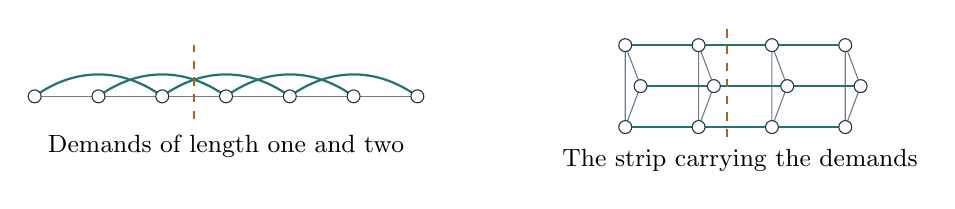
\begin{tikzpicture}[x=.81cm,y=.52cm,pt/.style={circle,draw=ink,fill=white,inner sep=1.65pt}]
\begin{scope}
\foreach \i in {0,...,6}{\coordinate (v\i) at (\i,0);}
\foreach \i in {0,...,5}{\pgfmathtruncatemacro{\j}{\i+1}\draw[ink!65] (v\i)--(v\j);}
\foreach \i in {0,...,4}{\pgfmathtruncatemacro{\j}{\i+2}\draw[sea,thick] (v\i) to[bend left=36] (v\j);}
\draw[ochre,dashed,thick](2.5,-.55)--(2.5,1.25);
\foreach \i in {0,...,6}{\node[pt] at (v\i) {};}
\node[below,font=\small] at (3,-.72) {Demands of length one and two};
\end{scope}
\begin{scope}[xshift=7.5cm]
\foreach \i in {0,...,3}{\foreach \j in {0,1,2}{\coordinate (p\i\j) at ({1.15*\i+.24*mod(\j,2)},{\j-.75});}}
\foreach \i in {0,...,3}{\draw[ink!65] (p\i0)--(p\i1)--(p\i2)--(p\i0);}
\foreach \i in {0,...,2}{\pgfmathtruncatemacro{\a}{\i+1}\foreach \j in {0,1,2}{\draw[sea,thick] (p\i\j)--(p\a\j);}}
\draw[ochre,dashed,thick] (1.6,-1.0)--(1.6,1.65);
\foreach \i in {0,...,3}{\foreach \j in {0,1,2}{\node[pt] at (p\i\j) {};}}
\node[below,font=\small] at (1.8,-1.05) {The strip carrying the demands};
\end{scope}
\end{tikzpicture}
\caption{On the left the three demands across the dashed cut occupy distinct coordinates. On the right all lanes across a layer cut carry the same vector, each with its share of the load.}\label{fig:strip}
\end{figure}

\begin{proof}[Proof of Proposition~\ref{prop:hard}]
Set \(M=d^2\) and \(c_e=\lceil M\|f_e\|\rceil\), omitting zero capacities. Extend \(Mf_e/c_e\) to a unit vector \(u_e\) by adding a private orthogonal coordinate. Projecting the outward sum to the demand coordinates gives \(Mb_v\). Hence \(\gamma\ge D=M\Gamma\).

A lane has vector norm at most \(\Gamma/d\), and a clique edge at most \(2\sqrt{2h}/d\). At a cut inside a layer there are at most \(d\) crossing lanes in total, some on each side of the layer, and at most \(d^2/4\) crossing clique edges. A table meets at most two lanes and \(d-1\) clique edges. Consequently
\[
 A\le M\Gamma+O(Md\sqrt h+d^2),\qquad
 T=O(M\Gamma/d+M\sqrt h+d).
\]
The hidden constants are absolute. Since \(d/\sqrt h=O(J^{-1/2})\), choose \(J\) so that the first inequality gives \(A\le(1+\eta)D\) for large \(d\). With this \(J\) fixed, \(D=\Theta_J(d^4)\), \(T=O_J(d^3)\), and \(B_0\le kT/2=O_J(d^5)\). There are \(O_J(d^3)\) output sites of norm \(1/2\). For \(L\) such sites, the Gaussian exponential moment gives \(\mathbb E\max\angles{g,x}\le \log(L)/z+z/8\) for \(z>0\), using natural logarithms here. Thus \(W(P)=O_J(\sqrt{\log d})\). Apply Lemma~\ref{lem:cost} with \(t=d^{-3/2}\). Its total error is \(O_J(d^{7/2}\sqrt{\log d})=o(D)\). The unweighted degree is at most \(d+1\), and a prefix crosses \(O(d^2)\) edges.
\end{proof}

\section{How many bits fit on the boundary?}\label{sec:transfer}

We use the same bookkeeping for all four polynomials. Fix \(m\), and suppose a block with \(m\) boundary positions can transmit \(\ell\ge1\) bits. The two tables at its ends may share \(m\) vertices, or have \(m\) edges joining the corresponding positions. To transmit a label means that after summing the private choices, the weight contributed between logical words \(i,j\in\bits^\ell\) is \(\one_{i=j}\). All graph weights may be specialized to constants, variables, or affine linear functions of single variables over \(\olF\). The original graph polynomials always have independent indeterminates over \(\F\).

\begin{lemma}\label{lem:transfer}
Split each edge of Proposition~\ref{prop:hard} into \(\lceil c_e/\ell\rceil\) blocks, padding its last word by zeros. Suppose the private graph for one table realizes its entries \(X_{v,\alpha}\), has size \(2^{O_m(T+d+1)}\), and can be swept with \(O_m(T+d+1)\) vertices in addition to the boundaries of unrelated blocks. Allow a constant number of additional vertices throughout the sweep. If such blocks exist with \(\liminf_{m\to\infty}\ell/m\ge\log_2 b\) along a sequence of \(m\)'s, then for each \(1<B<b\) there is a sequence of target graphs on which the circuit size \(s\) satisfies
\[
                    \frac{s}{n^C B^p}\longrightarrow\infty
\]
for every fixed \(C\ge0\). The pathwidths tend to infinity whenever the target has polynomial-size circuits on each class of bounded pathwidth.
\end{lemma}
\begin{proof}
Contraction of the equalities gives \eqref{eq:source}. Sweep in table order. Between tables keep the shared vertices of each crossing block or just its earlier edge endpoints. All blocks incident to the table being swept have \(O_m(T+d+1)\) positions in total. Rounding up the number of blocks costs at most \(m\) extra positions per crossing edge. Thus the target support has
\begin{equation}\label{eq:layout}
 p\le(m/\ell)A+O_m(d^2+T+d+1),\qquad \log_2 n=o(D).
\end{equation}
The last estimate follows by summing the size bound over \(k=Jd^2\) tables for fixed \(m,J\).

Here is the cost of specializing a border circuit. For a homogeneous degree-\(a\) target, keep degrees \(0,\ldots,a\) at each gate, convolving at products. This produces a circuit of size \(O((a+1)^2(s+1))\) for its degree-\(a\) part. Specialize its inputs and then take the degree-\(k\) component of the result. Coefficient specialization followed by extraction is linear on the bounded-degree coefficient spaces and hence preserves inclusion in the corresponding closures. The affine input substitutions cost \(O(n)\) gates, with constants depending on the fixed palette if present. Here \(a,k\le n^{O(1)}\). The same argument for ordinary border size simply specializes the bounded-degree outputs. Thus a target of size \(s\) yields source degree-component border size at most \(n^{O(1)}(s+1)\). This also explains why we may choose constants over \(\olF\).

Choose \(m\) with \((m/\ell)\log_2 B<1\), then \(\eta>0\) small enough that the strict inequality survives multiplication by \(1+\eta\). For these fixed choices, \eqref{eq:layout} gives \(p\log_2 B\le(1-\delta)D\) for some \(\delta>0\) and all large \(d\). By Proposition~\ref{prop:hard} and \(\log_2 n=o(D)\), the target has \(\log_2(s+1)\ge(1-o(1))D\), even in the stated border model. Subtracting \(C\log_2 n+p\log_2 B\) from \(\log_2(s+1)\) leaves at least \((\delta-o(1))D\), proving the ratio bound. If a subsequence had bounded pathwidth and hence polynomial-size circuits, its logarithmic circuit size would be \(O(\log n)=o(D)\). In particular, a target with upper bound \(n^{O(1)}2^{O(p)}\) must have \(p=\Omega(D)\) along this sequence, so \(\log n=o(p)\).
\end{proof}

\subsection{A table as a Boolean computation}

For matchings and tours it is convenient to implement a table once as a Boolean computation. Guess its incident label bits. In addition, one may guess a state of each incident block from a fixed finite set, check a fixed relation with its word, or give the pair a prescribed scalar weight. All the choices for one block depend only on \(m\). Check any padding and unused codewords. For each address \(\alpha\), in turn, compute the conjunction that the guessed bits spell \(\alpha\), and attach \(X_{v,\alpha}\) to the true value of this output. The weight of an accepted guess is the product of the weights of its true outputs. Exactly one address receives its variable. The address bits may stay live during the entire lookup. Testing the literals of a single address in sequence needs just a running conjunction. Even a table with \(2^T\) entries therefore has only \(O_m(T+d+1)\) simultaneously live bits. The total length, with wires counted, is \(2^{O_m(T+d+1)}\).

We need clauses that carry these weights into graph polynomials. For each Boolean gate, introduce one bit per row of its truth table and require exactly one row. For each incident bit \(x\) require exactly one of \(\neg x\) and the row bits in which \(x=1\). Unit clauses enforce constants and acceptance. Every guess that passes the checks has a unique extension. An exactly-one clause on literals \(z_1,\ldots,z_t\) can be replaced by ternary exactly-one clauses on \((a_{j-1},z_j,\neg a_j)\), with \(a_0=0\) and \(a_t=1\). Over Boolean values these enforce the integer identities \(a_j=a_{j-1}+z_j\). Give a weighted output a private copy \(b\) using the clause \((\neg x,b)\). Make these clauses at the time of their gate or output. Temporary row and prefix bits add constant live space per operation. In this clause order a bit is live from its first occurrence to its last. We use the same convention for a port bit whose end is attached to a block.

\section{Perfect matchings}

For even \(m\), a block has \(m\) possible matching edges between its two ends. We use exactly half of them. This provides \(\ell=\lfloor\log_2\binom m{m/2}\rfloor\) bits, since we may choose any \(2^\ell\) different half-sets. Although the partners of unused and used ports have different jobs, the following signed gadget lets all \(m\) ports at one end have the same bipartite color.

\begin{lemma}\label{lem:coupler}
In characteristic different from two, two prospective matching edges can be coupled to have total weight one when both or neither are used, and zero in all other boundary states.
\end{lemma}
\begin{proof}
Use three new rows and three new columns with internal weight matrix
\[
 Q=\begin{pmatrix}1/2&1/2&-1/2\\-1&-1&1\\1&1&1\end{pmatrix}.
\]
For prospective edge \(i\), \(i=1,2\), join its exterior row to new column \(i\) and new row \(i\) to its exterior column, both with weight one. An internal completion is the permanent of the submatrix left by the exterior choices. Different numbers of deleted rows and columns give zero. Direct expansion gives \(\per Q=1\), all four minors deleting one of the first two rows and one of the first two columns have permanent zero, and deleting both designated rows and columns leaves the entry \(1\). This also kills a choice entering at one port and leaving at the other.
\end{proof}

An even cycle has two alternating perfect matchings, representing the values of one bit. On its cycle reserve a distinct edge for every occurrence of a literal, present precisely when that literal is true. This is possible in any occurrence order by inserting unused edges until the desired parity is reached, then closing the cycle at even length. For a clause introduce a row and a column. For each of its literals couple the corresponding cycle edge to a prospective edge between this row and column, using a fresh copy of Lemma~\ref{lem:coupler}. The clause row and column support exactly one true occurrence after the private vertices have been summed out. An ordinary edge of a private output cycle, used precisely for true, receives its output weight. This realizes exactly the weighted verifier.

\paragraph{Completing a half-set.}
At the earlier table of a block put \(m\) terminals on the row side, and give them private column partners. Each terminal has its possible crossing edge and a prospective edge to its partner. Couple this private edge to an edge used for false on its port-bit cycle. Thus external use represents one. Add \(m/2\) dummy rows with a full \(m/2\) by \(m\) matrix of weights to the partners. For external set \(U\), the free partner columns are precisely \(U\). If \(|U|=m/2\), the completion weight \(P_U\) is the permanent of the corresponding square minor. Each such permanent contains distinct monomials with coefficient one. Their product is a nonzero polynomial. Choose weights in the infinite field \(\olF\) such that every \(P_U\ne0\). In the local lookup, reject unused words and attach the scalar \(1/P_U\) when choosing \(U\). Do the same with colors reversed at the later table. The crossing edges force the two subsets to coincide and give total weight one to each valid common word. The normalization works even when \((m/2)!\) vanishes in the field.

For the width bound, keep the initial vertex and the current end of the bit cycle for every live bit. Construct its occurrences in clause order. The next occurrence needs only a bounded number of new vertices, and the clause with its couplers is private to that step. All port and dummy graphs at one table together use \(O_m(T+d+1)\) vertices. A row of degree \(a>3\) can be split into two rows partitioning its neighbors, together with a new unit column adjacent to both rows. A matching uses one old edge and has a unique extension at this column. Repeat, and also split columns this way. At every clause or block the degrees to split are bounded in terms of \(m\), so the expansion preserves the local width and size estimates. Crossing terminals have degree two and need no expansion. Lemma~\ref{lem:transfer} applies because \(\binom m{m/2}\ge2^m/(m+1)\).

\paragraph{The matching upper bounds.}
Start and end a path decomposition with an empty bag, introducing or forgetting vertices one at a time. Process an edge once in a bag containing both endpoints. There are \(O(n)\) operations after removing redundant bags and scheduling the edges. Store a coverage bit at each live vertex. For an edge, either skip it or, if both ends are uncovered, cover them and multiply by its variable. Forget only covered vertices. At most \(2^{p+1}\) entries are needed. In characteristic two the signs of the determinant disappear. For completeness, a square matrix \(A\) of dimension \(a\) admits a division-free polynomial-size determinant circuit over any field. Eliminate on \(I+tA\) modulo \(t^{a+1}\) by successive diagonal pivots, all with constant term one. The coefficients of the inverse of a pivot follow successively from the product identity with \(1\). Thus all inverses use only polynomially many field operations on coefficients. The coefficient of \(t^a\) in the product of the pivots is \(\det A\). An unbalanced bipartite support has zero permanent. This proves Theorem~\ref{thm:permanent}.

\section{Directed tours}\label{sec:tours}

A boundary for a directed tour has \(m\) vertices shared by two tables. At each vertex specify which table supplies its incoming arc and which supplies its outgoing arc. Let \(U\) be the vertices at which a traversal leaves the left side and \(V\) those at which it enters the left side. They have equal size \(a\), and we use only patterns with \(a\ge1\). Assign each of the remaining \(m-2a\) vertices to the side that supplies both its arcs. The left table pairs \(V\) to \(U\) and the right table pairs \(U\) to \(V\). Once the two lists are numbered, the test for a single cycle is the matrix
\[
 H_a[\pi,\tau]=\one_{\pi\tau\text{ is an }a\text{-cycle}}\qquad(\pi,\tau\in S_a).
\]
Different degree patterns are incompatible. With common indexing for the patterns on the two sides, the full compatibility matrix \(K_m\) is therefore block diagonal. For each \(a\) it contains
\begin{equation}\label{eq:patterncount}
            \frac{m!\,2^{m-2a}}{a!^2(m-2a)!}
\end{equation}
copies of \(H_a\).

\begin{figure}[ht]
\centering
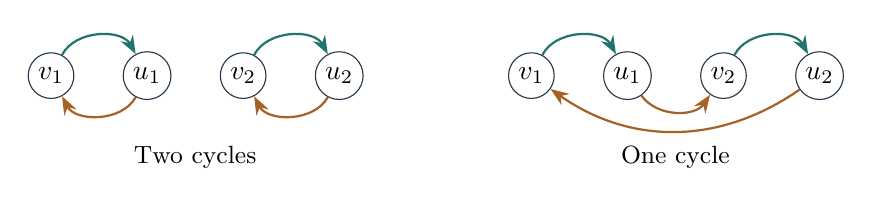
\begin{tikzpicture}[x=1cm,y=.65cm,>=Stealth,
 vert/.style={circle,draw=ink,fill=white,inner sep=2pt},
 leftpath/.style={sea,thick,->},rightpath/.style={ochre,thick,->}]
\foreach \i/\txt in {0/{v_1},1/{u_1},2/{v_2},3/{u_2}}{
 \node[vert] (v\i) at (\i*1.22,0) {\(\txt\)};
 \node[vert] (w\i) at (6.1+\i*1.22,0) {\(\txt\)};}
\foreach \n in {v,w}{
 \draw[leftpath] (\n0) to[bend left=62] (\n1);
 \draw[leftpath] (\n2) to[bend left=62] (\n3);}
\draw[rightpath] (v1) to[bend left=62] (v0);
\draw[rightpath] (v3) to[bend left=62] (v2);
\draw[rightpath] (w1) to[bend right=55] (w2);
\draw[rightpath] (w3) to[bend left=35] (w0);
\node[font=\small] at (1.83,-1.6) {Two cycles};
\node[font=\small] at (7.93,-1.6) {One cycle};
\end{tikzpicture}
\caption{The same left pairing (upper arcs) meets two different right pairings. For \(a=2\) the compatibility matrix has zeros on the diagonal and ones off the diagonal.}\label{fig:pairing}
\end{figure}

\subsection{How much rank is available?}

\begin{lemma}\label{lem:rank}
Over every field \(H_a\) contains a permutation submatrix of order \(2^{a-1}\). If the characteristic differs from two and \(a\) is nonzero in the field, then
\[
                     \rank H_a=\binom{2a-2}{a-1}.
\]
In particular, outside characteristic two \(\rank H_a\ge 4^a/a^{O(1)}\) for large \(a\).
\end{lemma}
\begin{proof}
Extend each permutation to fix \(a+1\), marking the extension with a hat, and put \(g=(a,a+1)\). Use rows \(\widehat\pi g^b\) and columns \(g^c\widehat\tau\) for \(b,c\in\bits\). If \(b=c\) the product fixes \(a+1\). Otherwise it inserts \(a+1\) in one old cycle and the test returns the old entry. This doubles the size of a permutation submatrix, starting with \(H_1=(1)\). It also embeds \(H_a\) in \(H_{a+1}\).

For the equality we may extend scalars to \(\olF\). On the subspace \(W=\{x\in\olF^a:\sum_i x_i=0\}\) the dot product is nondegenerate, since \(a\ne0\) in the field. A permutation \(\pi\) with cycle lengths \(d_1,\ldots,d_s\) has characteristic polynomial \(\prod_i(t^{d_i}-1)\). Removing the one trivial coordinate divides by \(t-1\). Evaluation at \(t=1\) therefore gives
\begin{equation}\label{eq:trace}
 \one_{\pi\ {\rm an}\ a\text{-cycle}}
   =a^{-1}\det(I-\pi|_W)
   =a^{-1}\sum_{j=0}^{a-1}(-1)^j\tr(\pi|_{\wedge^j W}).
\end{equation}
The last identity follows by expanding the determinant in principal minors.

We give the linear algebra showing that the group algebra acts on \(\bigoplus_j\wedge^j W\) as the full algebra \(\bigoplus_j\End(\wedge^j W)\). Write \(dA\) for the operator that applies \(A:W\to W\) to one factor at a time in a wedge and sums the results. For \(\alpha=e_i-e_j\), the transposition of \(i,j\) acts on \(W\) by \(I-\alpha\alpha^*\), where \(\alpha^*x=\angles{\alpha,x}\). Its action on the whole exterior algebra is \(I-d(\alpha\alpha^*)\), since two occurrences of \(\alpha\) in a wedge vanish. The image of the group algebra thus contains \(d(\alpha\alpha^*)\) for every root \(\alpha\). The roots \(\alpha_i=e_i-e_a\), \(i<a\), are a basis of \(W\). Taking their squares and those of \(\alpha_i-\alpha_j\) spans all symmetric operators, hence gives \(dA\) for every symmetric \(A\).

Choose an orthonormal basis of \(W\), using algebraic closedness and characteristic different from two. The commutator identity \([dA,dB]=d[A,B]\) follows by applying the operators to different wedge factors. From \(E_{ii}\) and \(E_{ij}+E_{ji}\) we obtain \(d(E_{ij}-E_{ji})\) by this identity, and then \(dE_{ij}\) by dividing by two. Here \(E_{ij}\) are the matrix units in the chosen basis. The operator \(dE_{ii}\) acts on a basis wedge by its indicator of containing index \(i\). Products of these operators and their complements therefore project onto \emph{individual} basis wedges across all degrees. Between two wedges of equal degree, successive one-index replacements by \(dE_{ij}\), with projections at the ends, realize any desired matrix unit up to sign. This proves the algebra assertion, including degrees zero and \(a-1\).

The matrix \(H_a\) represents the bilinear form \((x,y)\mapsto\varphi(xy)\) on the group algebra, where \(\varphi\) is the linear extension of \eqref{eq:trace}. On its image this is a sum of trace pairings on full matrix algebras with nonzero coefficients. Each trace pairing is nondegenerate, as can be seen on opposite matrix units. Pullback along a surjection preserves its rank. The rank is consequently \(\sum_j\binom{a-1}{j}^2=\binom{2a-2}{a-1}\). When the characteristic divides \(a\), apply the embedding from \(a-1\), which is then nonzero in the field. The central binomial estimate gives the final assertion.
\end{proof}

The characteristic-zero rank formula is also the bipartite connectivity formula of Raz and Spieker~\cite{rs,cln}. For our purposes set \(\rho=2\) in characteristic two and \(\rho=4\) otherwise. By Lemma~\ref{lem:rank}, \(\rank H_a\ge c\,\rho^a/(a+1)^C\) for absolute constants \(c,C>0\). Write \(R_m=\rank K_m\). Combining with \eqref{eq:patterncount} gives
\begin{equation}\label{eq:rankgrowth}
             R_m\ge (2+2\sqrt\rho)^m/m^{O(1)}\qquad(m\to\infty).
\end{equation}
Indeed, up to a polynomial factor the weighted sum is the constant coefficient of \((2+\sqrt\rho\,z+\sqrt\rho\,z^{-1})^m\), less \(2^m\) for \(a=0\). The coefficients are symmetric and largest at the center. To check the latter, a nonnegative symmetric unimodal sequence is a nonnegative sum of interval indicators centered at zero, and the convolution of two such indicators is symmetric unimodal. Here \(2\ge\sqrt\rho\). The center is at least the sum of all coefficients divided by \(2m+1\).

\subsection{Realizing the pairing test by a single tour}

We now construct the graph whose boundary has matrix \(K_m\). Every choice below on one side of a block is a function of that side's state only.

\paragraph{The prescribed paths.}
On each side lay down the paths of its pairing. On the first pair, in a fixed order, insert all vertices owned by that side for both arcs. Each of the other pairs is joined directly. On the left break the first arc \(x\to y\) of the first pair into \(x\to t_0\) and \(s_0\to y\) at two private vertices. When the two patterns agree, the joined paths give one spanning \(s_0\)-to-\(t_0\) path precisely when the unbroken pairings give one cycle. Any other cycle is confined to this block.

We must put \emph{all} choices in a single graph without leaving their unused private vertices uncovered. At each shared vertex \(v\), on each side, introduce two private vertices \(I_v,O_v\). Give the shared vertex the possible arcs \(I_v\to v\) and \(v\to O_v\). Route each prescribed local arc from the outgoing private vertex of its tail to the incoming private vertex of its head. Private terminals \(s_0,t_0\) use themselves at these connections. Call the private vertices used this way active. Prescribe a second, private path between two new terminals through \emph{all inactive} \(I_v,O_v\) on that side in fixed order. Use a direct connection if the list is empty. We will select exactly the private connections prescribed by this rule. Each inactive private vertex then has both degrees filled, and each active one forces its arc at \(v\). In particular, inconsistent patterns at a shared vertex cannot give a tour.

\paragraph{Selecting a connection.}
The table verifier guesses the state and computes a bit for each possible private connection indicating whether it was prescribed. Here is a directed version of the clause construction in Section~\ref{sec:transfer}. Represent a bit by a bidirected path, with forward traversal meaning true. In the clause order reserve a gap on the path for each literal. Put ordinary bidirected segments of length at least two between gaps and at either end. For a literal of clause \(C\), write its gap \(u,v\) in the direction that makes the literal true. Retain \(v\to u\) and replace \(u\to v\) by \(u\to C\to v\), where \(C\) is one vertex shared by the literals of the clause. Between successive bit paths put a connector accessible from either end of the first path and leading to either end of the next. Private start and end vertices make this entire verifier a segment. A private forward arc on each weighted bit path receives its weight.

In a spanning tour every ordinary segment has a consistent direction, since returning to the same neighbor at an interior vertex closes a two-cycle. At a gap, if one end requires the reverse arc \(v\to u\), that arc fills the corresponding need at both ends. Otherwise \(u\) needs its outgoing detour and \(v\) its incoming detour, forcing both arcs of the same literal. This prevents a tour from entering a clause through one occurrence and exiting through a different one. Each path has one direction and each clause is traversed exactly once. Conversely a satisfying assignment specifies the verifier traversal uniquely.

For a prospective private connection \(u\to v\) give its selection bit a private gap whose false-direction arc is \(x\to y\). Remove both prospective arcs. Introduce a fresh bidirected three-vertex path \(a,b,c\) and add
\[
                         u\to a,\quad c\to v,\quad x\to c,\quad a\to y .
\]
The reverse bit arc \(y\to x\) stays. The middle vertex \(b\) must use distinct neighbors, so a spanning tour traverses either \(u,a,b,c,v\) or \(x,c,b,a,y\), with a unique extension in either case. Contracting that path restores exactly one of the prospective arcs. In particular the bit traverses its false arc precisely when its private connection is unused. Surround the gap with ordinary segments just as for a clause occurrence.

Finally chain the verifier segments, the main segments \(s_0,t_0\), and all inactive-vertex path segments in one fixed cyclic order by their terminals. The main segment is attached at the earlier table, and each private segment at its own table. Order the attachments by table, so only a constant number of ends of this chain are ever live. For fixed local guesses, contracting all three-vertex paths leaves the prescribed block traversals and the verifier traversals. A tour exists precisely when every pattern agrees and each pairing closes one cycle before the break. When it exists it is unique. This proves the claimed compatibility matrix.

\paragraph{Using its rank.}
Put \(\ell=\lfloor\log_2 R_m\rfloor\). A nonsingular minor gives matrices \(U_0,V_0\) over the field with \(U_0K_m V_0=I_{2^\ell}\), by inverting the minor and restricting the identity. At each block end guess a physical state in addition to the logical word. If this is the left end, multiply by the corresponding entry of \(U_0\), and at the right end use \(V_0\). Each such entry can be emitted as a scalar weight of a true output when its word and state are guessed. Summing the guesses in the tour polynomial performs the matrix products, so the resulting logical block transmits equality. This construction uses a single graph even when some of the scalar entries are negative.

\paragraph{Width and degrees.}
Within one table all the blocks, relays, possible connections, and selection bits take \(O_m(T+d+1)\) vertices or bits before the serial lookup. Keep the endpoints of each bit path and one unfinished end during the clause sweep. Order the bit paths by first occurrence. The connectors between consecutive paths can then be installed when their endpoints are introduced, keeping the preceding path's endpoints until the next path starts, even if its clauses have already finished. This costs at most two extra vertices. Guards and clauses are generated at their occurrences. The width and size hypotheses of Lemma~\ref{lem:transfer} follow. Each shared vertex has indegree and outdegree at most two.

Here are details to bound the private degrees by three. A selector with one entry and \(b\) exits has a unique spanning path from its root to each chosen exit. To construct one, use a binary tree with the exits at its ordered leaves. Direct arcs from every internal node to its child roots. Give each child a representative leaf, and from that leaf add an arc to the other child root. A leaf represents itself. An internal subtree uses the rightmost leaf of its left child. Distinct internal subtrees determine distinct split gaps, so their chosen leaves are distinct. Each leaf supplies at most two crossing arcs and one external arc. Internal roots have at most two incoming and two outgoing arcs. A path ending in one child must first span the other, leave it through its representative, then span the desired child. Reentry into the first would revisit its root. Induction gives existence and uniqueness. Replace a high-degree private vertex by a reversed selector for its incoming arcs followed by a forward selector for its outgoing arcs. Their central arc is the only exit of the first and the only entry of the second. A spanning tour therefore traverses each selector just once. Keep old weights on the external arcs. At fixed \(m\) the affected private vertices have degree \(O_m(1)\), so the expansion preserves the layout. Equation~\eqref{eq:rankgrowth} and Lemma~\ref{lem:transfer} now give both directed lower bounds.

\subsection{Six states per vertex}

To match the lower bounds, first fix a root \(r\). A cycle cover is a selection of arcs using exactly one incoming and one outgoing arc at every vertex. After removing the arc out of \(r\), its remaining arcs form a tree oriented toward \(r\) precisely when the cover was a single tour. Work with basis vectors \(e_i\) for the vertices other than \(r\), and write \(e_r=0\). For each selected arc \(i\to j\) with \(i\ne r\), append \(e_i\) to one exterior product and \(e_i-e_j\) to a second. Multiply by the arc variable once, also for the selected arc out of \(r\).

For a complete cover, the coefficient in top degree of the two products together equals the determinant with columns \(e_i-e_j\) indexed by their tails. The first wedge supplies the sign for sorting the columns into tail order. If there is another cycle, its columns sum to zero. Otherwise order vertices by distance to the root. The matrix is triangular with diagonal one, so its determinant is one. Thus the weighted sum is exactly \(\hc(G)\).

On a path decomposition keep the current incoming and outgoing usage at each bag vertex. A basis wedge records which coordinates are occupied. In the first wedge this is already the outgoing usage. In the second, usage \(00\) implies unoccupied, since no incident arc has been taken. At usage \(11\) discard terms in which this coordinate is unoccupied, since no later column can fill it. Each mixed usage permits either occupancy. This gives \(1+1+2+2=6\) states per nonroot vertex. Forget only vertices with complete usage and, away from the root, complete occupancy. Order coordinates globally by forget time. Occupied forgotten coordinates make an initial segment in each wedge, so the sign for appending any coordinate is found by counting larger occupied live coordinates. A root has at most four states. Each arc thus costs polynomially many gates per entry and the bound is \(\OO(6^p)\) over any field.

\subsection{The smaller base in characteristic two}

We spell out the matching-basis update behind the characteristic-two algorithm of Cygan, Kratsch, and Nederlof~\cite{ckn}. It also explains why the same algorithm computes the formal polynomial with directed arcs and arbitrary characteristic-two weights.

Fix the outgoing arc \(u\to v\) of a root \(u\). We may assume there are at least two vertices and ignore loops. Delete that arc, introduce two new vertices \(s,t\), and force \(s\to v\) and \(u\to t\). A tour using the chosen arc corresponds to a spanning directed path from \(s\) to \(t\). Keep \(s,t,u,v\) available from the outset, adding at most four to the width. Initialize with the two forced arcs, and require all original vertices eventually to have one incoming and one outgoing arc. In the undirected view of a partial selection, its nontrivial components are paths, apart from premature cycles which we discard. Antiparallel arcs are separate edge choices, so a doubled undirected edge can be a two-cycle.

For a fixed vector of oriented degrees let \(E_1\) be the set of degree-one vertices, including \(s,t\), of even size \(b\ge2\). Each path joins a pair of \(E_1\). For a test matching \(M\) on \(E_1\), let \(T(M)\) sum the weights of the partial selections whose paths together with \(M\) close into one cycle. Unused live vertices have degree zero and are ignored by the test. Closed components in the partial selection give zero for every test, since \(s,t\) are endpoints. Once all original vertices are complete the only test is \(st\), so its value is the desired path sum.

Order the \(b\) endpoints. Divide them into a first singleton, successive pairs, and a last singleton. Use as \emph{chain tests} precisely the matchings with one edge between each two successive groups. Each pair group chooses which vertex receives the edge from the preceding group. There are \(2^{b/2-1}\) tests. We show how to process an arc in polynomial work per stored test.

\begin{lemma}\label{lem:localbasis}
On \(j=2,4,6\) sites every matching test is, in characteristic two, a linear combination of the chain tests in any prescribed order. This remains true with an arbitrary fixed collection of paths attached outside the sites, provided every site has one free end.
\end{lemma}
\begin{proof}
Index the rows and columns of a matrix \(H\) by perfect matchings of the sites. Set \(H[P,M]=1\) when their union is one cycle, counting a doubled edge as a cycle on two sites. We show that the columns for the chain tests span \(H\). On two sites there is just one matching. On four sites two different matchings close one cycle. Each row therefore contains two ones, so the three columns sum to zero in characteristic two. The two chain columns are independent, since on their own rows one reads \((0,1)\) and the other \((1,0)\).

On six sites two matchings close one cycle precisely when they are edge-disjoint. Consider the partitions of the edges of \(K_6\) into five perfect matchings. Every disjoint pair lies in exactly one such partition. Indeed, removing its six-cycle leaves two triangles joined by three disjoint edges. Each of the three remaining perfect matchings must use one joining edge. That edge determines the other two edges of its matching, one in each triangle.

A fixed perfect matching \(P\) has eight disjoint partners. Of the fifteen matchings, one is \(P\), and six others share one of its three edges. Each partition containing \(P\) accounts for four partners, so \(P\) belongs to two partitions. Counting incidences now gives \(15\cdot 2/5=6\) partitions in total. Let \(v_P\in\F^6\) indicate the two containing \(P\). In characteristic two,
\[
                         H[P,M]=\langle v_P,v_M\rangle .
\]
The dot product is one for a disjoint pair. Distinct matchings sharing an edge lie in no common partition, and for \(P=M\) the dot product is \(1+1=0\). Each \(v_P\) lies in the five-dimensional subspace of coordinate sum zero. The all-ones vector belongs to this subspace and annihilates it, so the restricted dot product has rank at most four. Hence \(\rank H\le4\).

There are four chain matchings on six sites. Two of them are edge-disjoint exactly when their choices at both middle pairs are opposite. An agreement gives the same edge at the first or last singleton, and two opposite choices leave all three edges different. Their four columns thus restrict to a permutation matrix on their four rows. They are independent and span \(H\). In all three sizes the restriction to the chain rows gives the coefficients of any desired test up to this permutation. For fixed outside paths, a separate cycle makes all tests zero. Otherwise the paths contract to a matching \(P\) on the free ends, so the same column identity applies to each completion and hence to every weighted sum.
\end{proof}

First, one may swap adjacent vertices in the order with constant work per new test. If the vertices belong to different groups, freeze all edges of the new test outside those two groups, leaving one exposed endpoint at each neighboring group that exists. At most six sites remain. The old tests extending the frozen edges restrict to exactly the chain tests on these sites, in their old order. Lemma~\ref{lem:localbasis} expresses the desired test using them. A swap within one group merely permutes the tests. Thus any reorder costs polynomial work per entry.

To introduce the arc \(i\to j\), either skip it, or take it when the two oriented degrees allow this. Move the affected endpoints to the end in the old and new orders, using adjacent swaps. For the take transition, pull a new test back across the arc. Place the undirected edge \(ij\) beside the new test and suppress vertices of degree two in this complementary collection. This leaves a matching on the old endpoints, unless it forms a closed complementary component, in which case the contribution is zero because the forced endpoints are elsewhere. More explicitly, two newly created endpoints are spliced out of their test edges, a single new endpoint is replaced by the endpoint that disappeared, and two disappearing endpoints are matched directly. This operation has exactly the one-cycle test of adding the arc to the partial paths.

The untouched endpoints form a common prefix in both orders and include \(s,t\). Take its longest odd-length initial part. In a chain test its internal edges leave one exposed vertex. Freeze those edges. The remaining local sites for the pulled-back test are this exposed vertex, at most one further untouched endpoint, and at most the two affected endpoints. The old chain tests with these frozen edges realize all chain tests on the remaining two or four sites. Lemma~\ref{lem:localbasis} again gives a constant-size update. Multiply the take transition by the arc variable and add it to the proper degree vector, restoring the original order. Introducing an unused vertex leaves every test unchanged. Forgetting an original vertex requires complete degrees, so it is absent from the endpoint list.

If \(b\) endpoints are mixed, the number of stored tests is at most \((\sqrt2)^b\). At each ordinary bag vertex the two neutral types \(00,11\) have factor one and each of the two mixed types has factor \(\sqrt2\). Summing over degree vectors gives \((2+2\sqrt2)^{p+O(1)}\) entries. Adjacent reorders, the choice of the root arc, and all bag operations give only polynomial factors. Multiply the final path sum by the deleted arc's variable and sum over the possible root arcs. Every tour occurs once. This finishes Theorem~\ref{thm:tours}.

\section{The Tutte cluster polynomial and its coloring specializations}\label{sec:color}

For a positive integer \(q\), distribute each edge factor to get
\begin{equation}\label{eq:potts}
 Z_G(q,\mathbf w)=\sum_{\sigma:V\to[q]}
               \prod_{uv\in E}\bigl(1+w_{uv}\one_{\sigma(u)=\sigma(v)}\bigr).
\end{equation}
Indeed, selecting the second summand on \(A\) forces one common color per component of \((V,A)\), giving the coefficient in \eqref{eq:cluster}. In particular \(w_e=-1\) tests disequality and \(w_e=0\) removes the edge. For every positive integer \(q\) this gives the coloring count on the chosen subgraph. Equality at all such integers identifies the chromatic polynomial over \(\mathbb Z[Q]\), hence also after reduction to any field. A multilinear polynomial in the edge indicators is determined on the Boolean cube, by successively taking its values at zero and one in each variable.

There is a second useful Boolean interpretation. To interpolate the \emph{cluster weight} \(A\mapsto Q^{\kappa(V,A)}\) itself, use the random-cluster normalization
\begin{equation}\label{eq:normalized}
 \sum_{A\subseteq E}Q^{\kappa(V,A)}
       \prod_{e\in A} y_e\prod_{e\notin A}(1-y_e)
    =\prod_{e\in E}(1-y_e)\,Z_G\!\left(Q,\left(\frac{y_e}{1-y_e}\right)_{e\in E}\right).
\end{equation}
This is a polynomial identity after clearing denominators. For a single edge the standard form is \(Q^2+Qw\), the chromatic extension is \(Q^2-Qy\), and the normalized cluster weight is \(Q^2(1-y)+Qy\). The inverse change in \eqref{eq:normalized} sends \(y_e\) to \(w_e/(1+w_e)\) and multiplies by \(\prod_e(1+w_e)\). Both changes preserve the circuit bounds up to polynomial factors. Indeed scale all new edge variables by an auxiliary \(z\), expand the unit denominators modulo \(z^{|E|+1}\), multiply in that truncated ring at each gate, and finally sum the coefficients. The desired output has edge degree at most \(|E|\). The same bounded coefficient transformation preserves border bounds.

\subsection{A table of named colors}

We first allow each vertex to distinguish the colors by assigning them separate variables. One boundary vertex can then carry any of \(q\) symbols.

Let \(\F\) be any field and \(q\ge1\) a fixed integer. For a loopless undirected graph \(G=(V,E)\) of pathwidth \(p\), put \(n=1+|V|+|E|\) and give each vertex-color pair its own variable. The proper-coloring polynomial with these activities is
\begin{equation}\label{eq:list}
 L_{G,q}(\mathbf x)=\sum_{\substack{\sigma:V\to[q]\\\sigma\ \mathrm{proper}}}
                      \prod_{v\in V}x_{v,\sigma(v)} .
\end{equation}

\begin{proposition}[Named vertex colors]\label{prop:named}
If \(q\ge3\), then for every \(0<\varepsilon<q-1\) and \(C\ge0\) there are graphs of arbitrarily large \(p\) with \(s_{\F}(L_{G,q})>n^C(q-\varepsilon)^p\), and \(n^{O(1)}q^p\) gates suffice for every graph. If \(q\le2\), polynomial-size circuits suffice for every graph.
\end{proposition}

For example, three named colors over \(\F_2\) give base three. On the same support \(Z_G(3,\mathbf w)=\prod_e(1+w_e)\). Over \(\mathbb Q\), two named colors give a polynomial-size circuit on every graph, while the two-color cluster polynomial has base two. To prove the proposition we shall specialize \(L_{G,q}\) to an arbitrary table of boundary colors. A short path suffices to test the implication that we need.

\begin{lemma}\label{lem:implication}
Let \(q\ge3\). Give a switch \(s\) a list of two distinct colors, called off and on, and let \(v\) be a vertex with the full palette. For each prescribed color \(a\), a constant-size list-coloring graph with scalar activities realizes the factor
\[
 [s=\mathrm{off}]+[s=\mathrm{on}]\,[v=a].
\]
Its two endpoint weights may be multiplied into any existing activities.
\end{lemma}
\begin{proof}
We first forbid one pair \((v=c,s=\mathrm{on})\). If \(c\ne\mathrm{on}\), take the sequence of colors \(c,t,\mathrm{on}\) with \(t\) distinct from the other two. If \(c=\mathrm{on}\), take \(c,t,u,c\) with \(c,t,u\) distinct. Put a path between \(v\) and \(s\) with one internal vertex for each consecutive pair of colors in the sequence, giving that vertex the pair as its list. An endpoint color \(v=c\) forces successive internal vertices to take the right member of their pair, ending with \(\mathrm{on}\). It extends precisely when \(s\ne\mathrm{on}\). For \(v\ne c\), take left members up to the penultimate internal vertex. Both colors at the last vertex differ from the preceding choice, so at least one also differs from \(s\). Lists are implemented by setting the activities of other colors to zero.

Use such a path for every \(c\ne a\), with disjoint interiors. Give every allowed internal vertex-color pair its own formal activity. For any extendible endpoint assignment the sum of internal weights is a nonzero polynomial, since different extensions give different monomials. Specialize simultaneously so that all those values stay nonzero in \(\olF\). Denote the resulting factor by \(g(s,v)\). It is nonzero for \((\mathrm{off},b)\) at every \(b\), and in the on row exactly at \(b=a\). Multiply the activity of color \(b\) at \(v\) by \(1/g(\mathrm{off},b)\) and the on activity at \(s\) by \(g(\mathrm{off},a)/g(\mathrm{on},a)\). The three possible kinds of entries now have the stated values.
\end{proof}

\begin{example}
With colors red, blue, green, a path from \(v\) to \(s\) with internal lists \(\{\text{red},\text{green}\}\) and \(\{\text{green},\text{blue}\}\) forbids exactly the pair \(v=\text{red},s=\text{blue}\). If \(v\) is red, the interior is forced to be green, blue in that order. This is the only endpoint assignment that cannot extend when \(s\) is blue.
\end{example}

\paragraph{Reading the table.}
Use \(m\) shared vertices per block to represent \(\ell=\lfloor m\log_2 q\rfloor\) bits by distinct words. Retain all boundary positions of the current table. If it has \(b\) positions, scan all \(\tau\in[q]^b\). Let \(Y_\tau=X_{v,\alpha}\) if the words at the positions decode to a valid joint address \(\alpha\), and \(Y_\tau=0\) otherwise. For this \(\tau\) introduce a switch of off weight one and on weight \(Y_\tau-1\). Use Lemma~\ref{lem:implication} between it and each position, prescribing the color \(\tau_i\). Given an actual boundary assignment \(z\), summing the switch gives
\[
                      1+(Y_\tau-1)\one_{z=\tau}.
\]
Multiplying over all \(\tau\) leaves exactly \(Y_z\). All endpoint scalar normalizations multiply into the appropriate activities, also when a boundary vertex serves two tables. Retain one switch at a time and sweep its constant-size paths. There are \(b=O_m(T+d+1)\) positions, which proves both local bounds of Lemma~\ref{lem:transfer}. The usual dynamic program stores one color per bag vertex, multiplies its activity once, and tests each edge once. This gives \(\OO(q^p)\). For \(q=2\) each connected bipartite component has precisely the two colorings given by its bipartition. Its polynomial is a sum of two monomials, and one multiplies over components. A nonbipartite component gives zero. The case \(q=1\) follows directly from \eqref{eq:list}. This proves Proposition~\ref{prop:named}.

\subsection{Fixing the cluster parameter}
By \eqref{eq:cluster}, \(Z_G(q,\mathbf w)=Z_G(r,\mathbf w)\) with \(r\) as in Theorem~\ref{thm:color}. For nonempty \(V\) it vanishes at \(r=0\), and equals \(\prod_e(1+w_e)\) at \(r=1\). The empty graph gives one. For \(r\ge2\), keeping one of \(r\) colors per live vertex and multiplying the factors of \eqref{eq:potts} gives \(\OO(r^p)\).

For \(r\ge3\), introduce an \(r\)-clique of anchors and give its edges weight \(-1\). Make every vertex \(v\) of the named model adjacent to every anchor \(i\) with weight \(x_{v,i}-1\). Set each original properness edge to \(-1\). The anchors use all colors. Relative to their order, an assignment at \(v\) receives exactly its prescribed activity. There are \(r!\) assignments to the anchors, and \(r!\) is invertible because \(r\) is smaller than the positive characteristic when the characteristic is nonzero. This recovers \(L_{G,r}\) after division by \(r!\). The anchors add at most \(r\) to the width. They work just as well if the original edges have arbitrary weights.

The last case is \(r=2\). These same anchors allow arbitrary unary weights. An edge with \(w=a-1\) contributes \(a\) on equal spins and one otherwise. Take two such edges in series with equal-spin weights \(a,b\), and give their middle spin unary weights \((-ab,1)\). Summing the middle spin gives, in the order \(0,1\) at both ends,
\[
 \begin{pmatrix}a&1\\1&a\end{pmatrix}
 \begin{pmatrix}-ab&0\\0&1\end{pmatrix}
 \begin{pmatrix}b&1\\1&b\end{pmatrix}
 =
 \begin{pmatrix}1-a^2b^2& b(1-a^2)\\ a(1-b^2)&0\end{pmatrix}.
\]
Choose \(a,b\in\olF\) so that the three entries outside the bottom right corner are nonzero. Row and column scalings can turn them all into ones, since their support is a tree on the two row and two column indices. A hard disequality edge to a fresh spin flips an index uniquely. We can therefore forbid any one corner and realize either implication between a switch and a prescribed bit. The preceding table lookup now works with \(m\) bits on \(m\) shared vertices. Add the two anchors only once for the whole graph. The affine substitutions and constant width overhead satisfy Lemma~\ref{lem:transfer}. Finally the change \(w_e=-y_e\) costs at most \(|E|\) gates in either direction, which the ratio bound in that lemma absorbs. This proves Theorem~\ref{thm:color}.

\subsection{An indeterminate cluster parameter}

When \(Q\) is free we can let the palette grow. In small characteristic its factorial may vanish. We first show how to recover all named activities even then. Write \((Q)_a=Q(Q-1)\cdots(Q-a+1)\).

\begin{lemma}\label{lem:anchors}
Take any graph with \(a\) named colors and activities. Add \(a\) anchors with the weights used above, and write \(F(Q)\) for the resulting specialization of the cluster polynomial. There is a polynomial \(U\) such that
\[
 F(Q)=(Q)_a U(Q),\qquad U(a)=L_{G,a} .
\]
The identities hold over every field. A circuit of size \(s\) for the cluster polynomial yields a circuit for \(L_{G,a}\) with \(O((a+1)^2(s+n+1))\) gates after the indicated affine substitutions.
\end{lemma}
\begin{proof}
Work first over the integers with independent activities. For each integer \(u\ge a\), \eqref{eq:potts} permits \((u)_a\) ordered assignments to the anchors. Given their colors, describe an extension by its vertices in each named color and by a partition of the remaining vertices into \(j\) nonempty outside color classes. These classes can be labeled in \((u-a)_j\) ways. Each description has a weight independent of \(u\). Thus \(U(Q)=\sum_j (Q-a)_j U_j\) is a polynomial over the integers in \(Q\) and the activities, and \(U_0=L_{G,a}\). Equality at all integers \(u\ge a\) proves the identity. It survives reduction and specialization.

In the coefficient field write \((a+z)_a=z^h(c+O(z))\) with \(c\ne0\). Here \(h\le a\) is just the number of zero constant factors. Then \(U(a)=c^{-1}[z^h]F(a+z)\). Computing at each gate modulo \(z^{h+1}\) costs \(O((h+1)^2)\) operations. The procedure also applies in border complexity by linearity on the bounded-degree coefficient spaces.
\end{proof}

\begin{proof}[Proof of Theorem~\ref{thm:cluster}]
For the upper bound, keep a partition of the bag according to connectivity by selected edges. Introduce a vertex as a singleton. At an edge either skip it, or merge the endpoint classes and multiply by \(w_e\). On forgetting the last vertex of a class, multiply by \(Q\). Every selected edge set then contributes precisely its term in \eqref{eq:cluster}. The number of states is at most \(\operatorname{Bell}(p+1)\le(p+1)^{p+1}\).

For the lower bound use the strip of Proposition~\ref{prop:hard}, with \(J\) fixed after \(\eta\), and take \(a=\lfloor D/(\log_2 D)^3\rfloor\) named colors. Put \(\ell=\lfloor\log_2 a\rfloor\) bits on \emph{one} shared vertex of each block. At a table there are at most \(b\le T/\ell+d+1\) such positions. The lookup uses \(a^b\) switches. For each position, its paths in Lemma~\ref{lem:implication} can be processed one at a time, each with at most three internal vertices, even as \(a\) grows. Keep the \(b\) positions, the current switch, and all \(a\) anchors. Their clique edges add no more vertices to a bag. Including the \(O(d^2)\) rounding cost for crossing edges, we obtain
\[
 p\le A/\ell+O(d^2+b+a+1)\le (1+\eta+o(1))D/\log_2 D .
\]
The constant in the first \(O\) is absolute. There are at most polynomially many vertices and edges in \(k,a,b\) times \(a^{\max b}\), since each switch uses \(O(ab)\) short paths and each vertex meets at most \(a\) anchors in addition to the named graph edges. Hence \(\log_2 n=O_J(T+d\log a+\log D)=o(D)\). Lemma~\ref{lem:anchors} extracts the source with a polynomial factor in \(n\), uniformly in \(a\). Proposition~\ref{prop:hard} gives \(\log_2(s+1)\ge(1-o(1))D\) for target size \(s\). In particular the pathwidth tends to infinity, by the upper bound. Given \(0<\varepsilon<1\), choose \(\eta\) so that \(\delta=1-(1-\varepsilon)(1+\eta)>0\). Since \(p\log_2 p\le(1+\eta+o(1))D\), subtracting \(C\log_2 n+(1-\varepsilon)p\log_2 p\) from \(\log_2(s+1)\) leaves at least \((\delta-o(1))D\) for every fixed \(C\). This gives the stated strict gate lower bound.
\end{proof}

\clearpage
\section{An open question}

Can the permanent in characteristic different from two, or the directed Hamiltonian cycle polynomial in any characteristic, be shown to require \(2^{\Omega(N)}\) arithmetic gates as a function of the matrix order \(N\) alone? OpenAI proved a superpolynomial lower bound in this parameter~\cite{circuits}. Our constructions use a separate variable for each entry of a local table. An exponential bound in matrix order would require controlling how many entries suffice for a given circuit lower bound, or a different source of hardness. For the permanent the counting-stars algorithm already gives an upper bound with base strictly below two in matrix order~\cite{stars}.

\bibliographystyle{../linkedtitles}
\bibliography{../references}
\end{document}
